\subsection{Strategic Advantage Condition in Regression}
\label{sec:regression}

The outcome space $\cY = \R$ is the space of real numbers and the loss function $\ell(y, \yhatm) = (y - \yhatm)^2$ is mean squared error (MSE). For this regression formulation, we explicitly assume that all random variables ($U, X, Y$) have zero mean everywhere. In the mandatory disclosure setup, the Sender always chooses $A=x$. For a linear Receiver strategy $\yhatvemt = 0$ and $\yhatvx = b^\top x$, we characterize the resulting risk in the following lemma.

\begin{lemma} \label{lem:rv_regression} In the mandatory disclosure setup, for a Receiver strategy parameterized by $b \in \R^d$, the expected risk is
\begin{align}
R_V(b, q) = \Var(Y) & - (1-q) \Var(b_Y^\top X) \nonumber \\
& + (1-q)\Var((b-b_Y)^\top X), \label{eq:rv_b}
\end{align}
where $b_Y = \Var(X)^{-1}\Cov(X,Y)$. The optimal vanilla risk is achieved at $b = b_Y$, yielding
\begin{equation}
R_V^\star(q) = \Var(Y) - (1-q) \Var(b_Y^\top X).
\end{equation}
\end{lemma}

\begin{remark}
Note that $b_Y = \Var(X)^{-1}\Cov(X,Y)$ is the optimal weight vector for ordinary least squares (OLS) regression of $Y$ on $X$.
\end{remark}

In the voluntary disclosure setup, for a given Receiver strategy $\yhatm$, we consider the linear form $\yhatempt = 0$ and $\yhatx = b^\top X$, where $b \in \R^d$. For a fixed $b$, we define the following scalar fields:
\begin{align}
F(x,u) &:= (2u - b^\top x) b^\top x, \\
G(x,y) &:= (2y - b^\top x) b^\top x.
\end{align}
The Sender's best response action is then characterized by the following lemma.

\begin{lemma} \label{lem:sender_response}
  In the voluntary disclosure setup, for a given receiver strategy $\yhatm$, the Sender's best response action is given by
  \begin{equation}
    A(x,u) = x \iff F(x,u) > 0.
  \end{equation}
\end{lemma}

Based on this best response, we derive the Receiver's strategic risk $R_S$ in the next lemma.

\begin{lemma} \label{lem:rs_regression}
  Given a Receiver strategy $\yhatm$ parameterized by $b$, the resulting strategic risk is
  \begin{equation}
    R_S(b, q) = \Var(Y) - (1-q)\E[G(X,Y)\Ind{F(X,U) > 0}],
  \end{equation}
  where $\Ind{\cdot}$ denotes the indicator function.
\end{lemma}

\begin{remark}
The Stackelberg equilibrium risk is defined as the minimum strategic risk over the parameter space:
\begin{equation*}
  R_S^\star(q) := \min_b R_S(b, q).
\end{equation*}
\end{remark}

\begin{remark}
The function $F(x,u)$ serves as the decision rule for the Sender. The function $G(x,y)$ represents the Receiver's gain when the feature vector $x$ is successfully received through the noisy channel (i.e., the signal is not lost to noise) relative to when the feature vector is lost.
\end{remark}

The strategic advantage condition is $R_V^\star(q) - R_S^\star(q) > 0$. We provide a sufficiency condition for this inequality in the following theorem.

\begin{theorem}[Sufficiency Condition] \label{thm:sufficiency_reg}
  A strategic advantage exists if there exists $b \in \R^d$ such that:
\begin{align}
    \|U{-}Y\|_2 
    &< 
    \frac{\E\big[| G(X,Y)|\big] 
    - \Var(b_Y^\top X)}{4\sqrt{\Var(b_Y^\top X)}} \nonumber \\
    &\quad - \frac{\Var((b{-}b_Y)^\top X)}{4\sqrt{\Var(b_Y^\top X)}}, \label{eq:sufficiency_reg}
\end{align}
  where $\|U{-}Y\|_2 = \sqrt{\Var(U) + \Var(Y) - 2 \Cov(U,Y)}$, $b_Y = \Var(X)^{-1}\Cov(X,Y)$, and $G(X,Y) = (2Y - b^\top X) b^\top X$.
\end{theorem}

Beyond sufficiency, we can also identify a necessary condition for a strategic advantage to be possible. We define a strategic disadvantage when $R_S^\star(q) = R_V^\star(q)$; therefore, a necessary condition for an advantage must be the complement of this state.

\begin{theorem}[Necessary Condition] \label{thm:necessary_reg}
  A necessary condition for a strategic advantage to exist is:
  \begin{align}
    \max_b \Big( \E\big[| G(X,Y)|\big] &- \Var(b_Y^\top X) \nonumber \\
    &- \Var((b{-}b_Y)^\top X) \Big) > 0. \label{eq:necessary_reg}
  \end{align}
\end{theorem}

\begin{remark}
The necessary condition in \eqref{eq:necessary_reg} is equivalent to the requirement that the sufficiency condition in \eqref{eq:sufficiency_reg} be non-vacuous. Since the left-hand side of \eqref{eq:sufficiency_reg} is non-negative, the condition in \eqref{eq:necessary_reg} is equivalent to the numerator on the right-hand side being positive (as the denominator is always positive), thereby allowing for the existence of a non-empty range for $\|U-Y\|_2$.
\end{remark}

\begin{remark}
Both the necessary and sufficient conditions are independent of the channel noise parameter $q$. This highlights that channel noise only controls the magnitude of the strategic advantage, not whether it can be attained. Additionally, both theorems require the bounds to hold for the best possible parameter $b$. Consequently, if the conditions are satisfied evaluated simply at the vanilla optimal weight $b_Y$, they necessarily hold under optimal $b$.
\end{remark}

\begin{figure}[htpb]
  \centering
  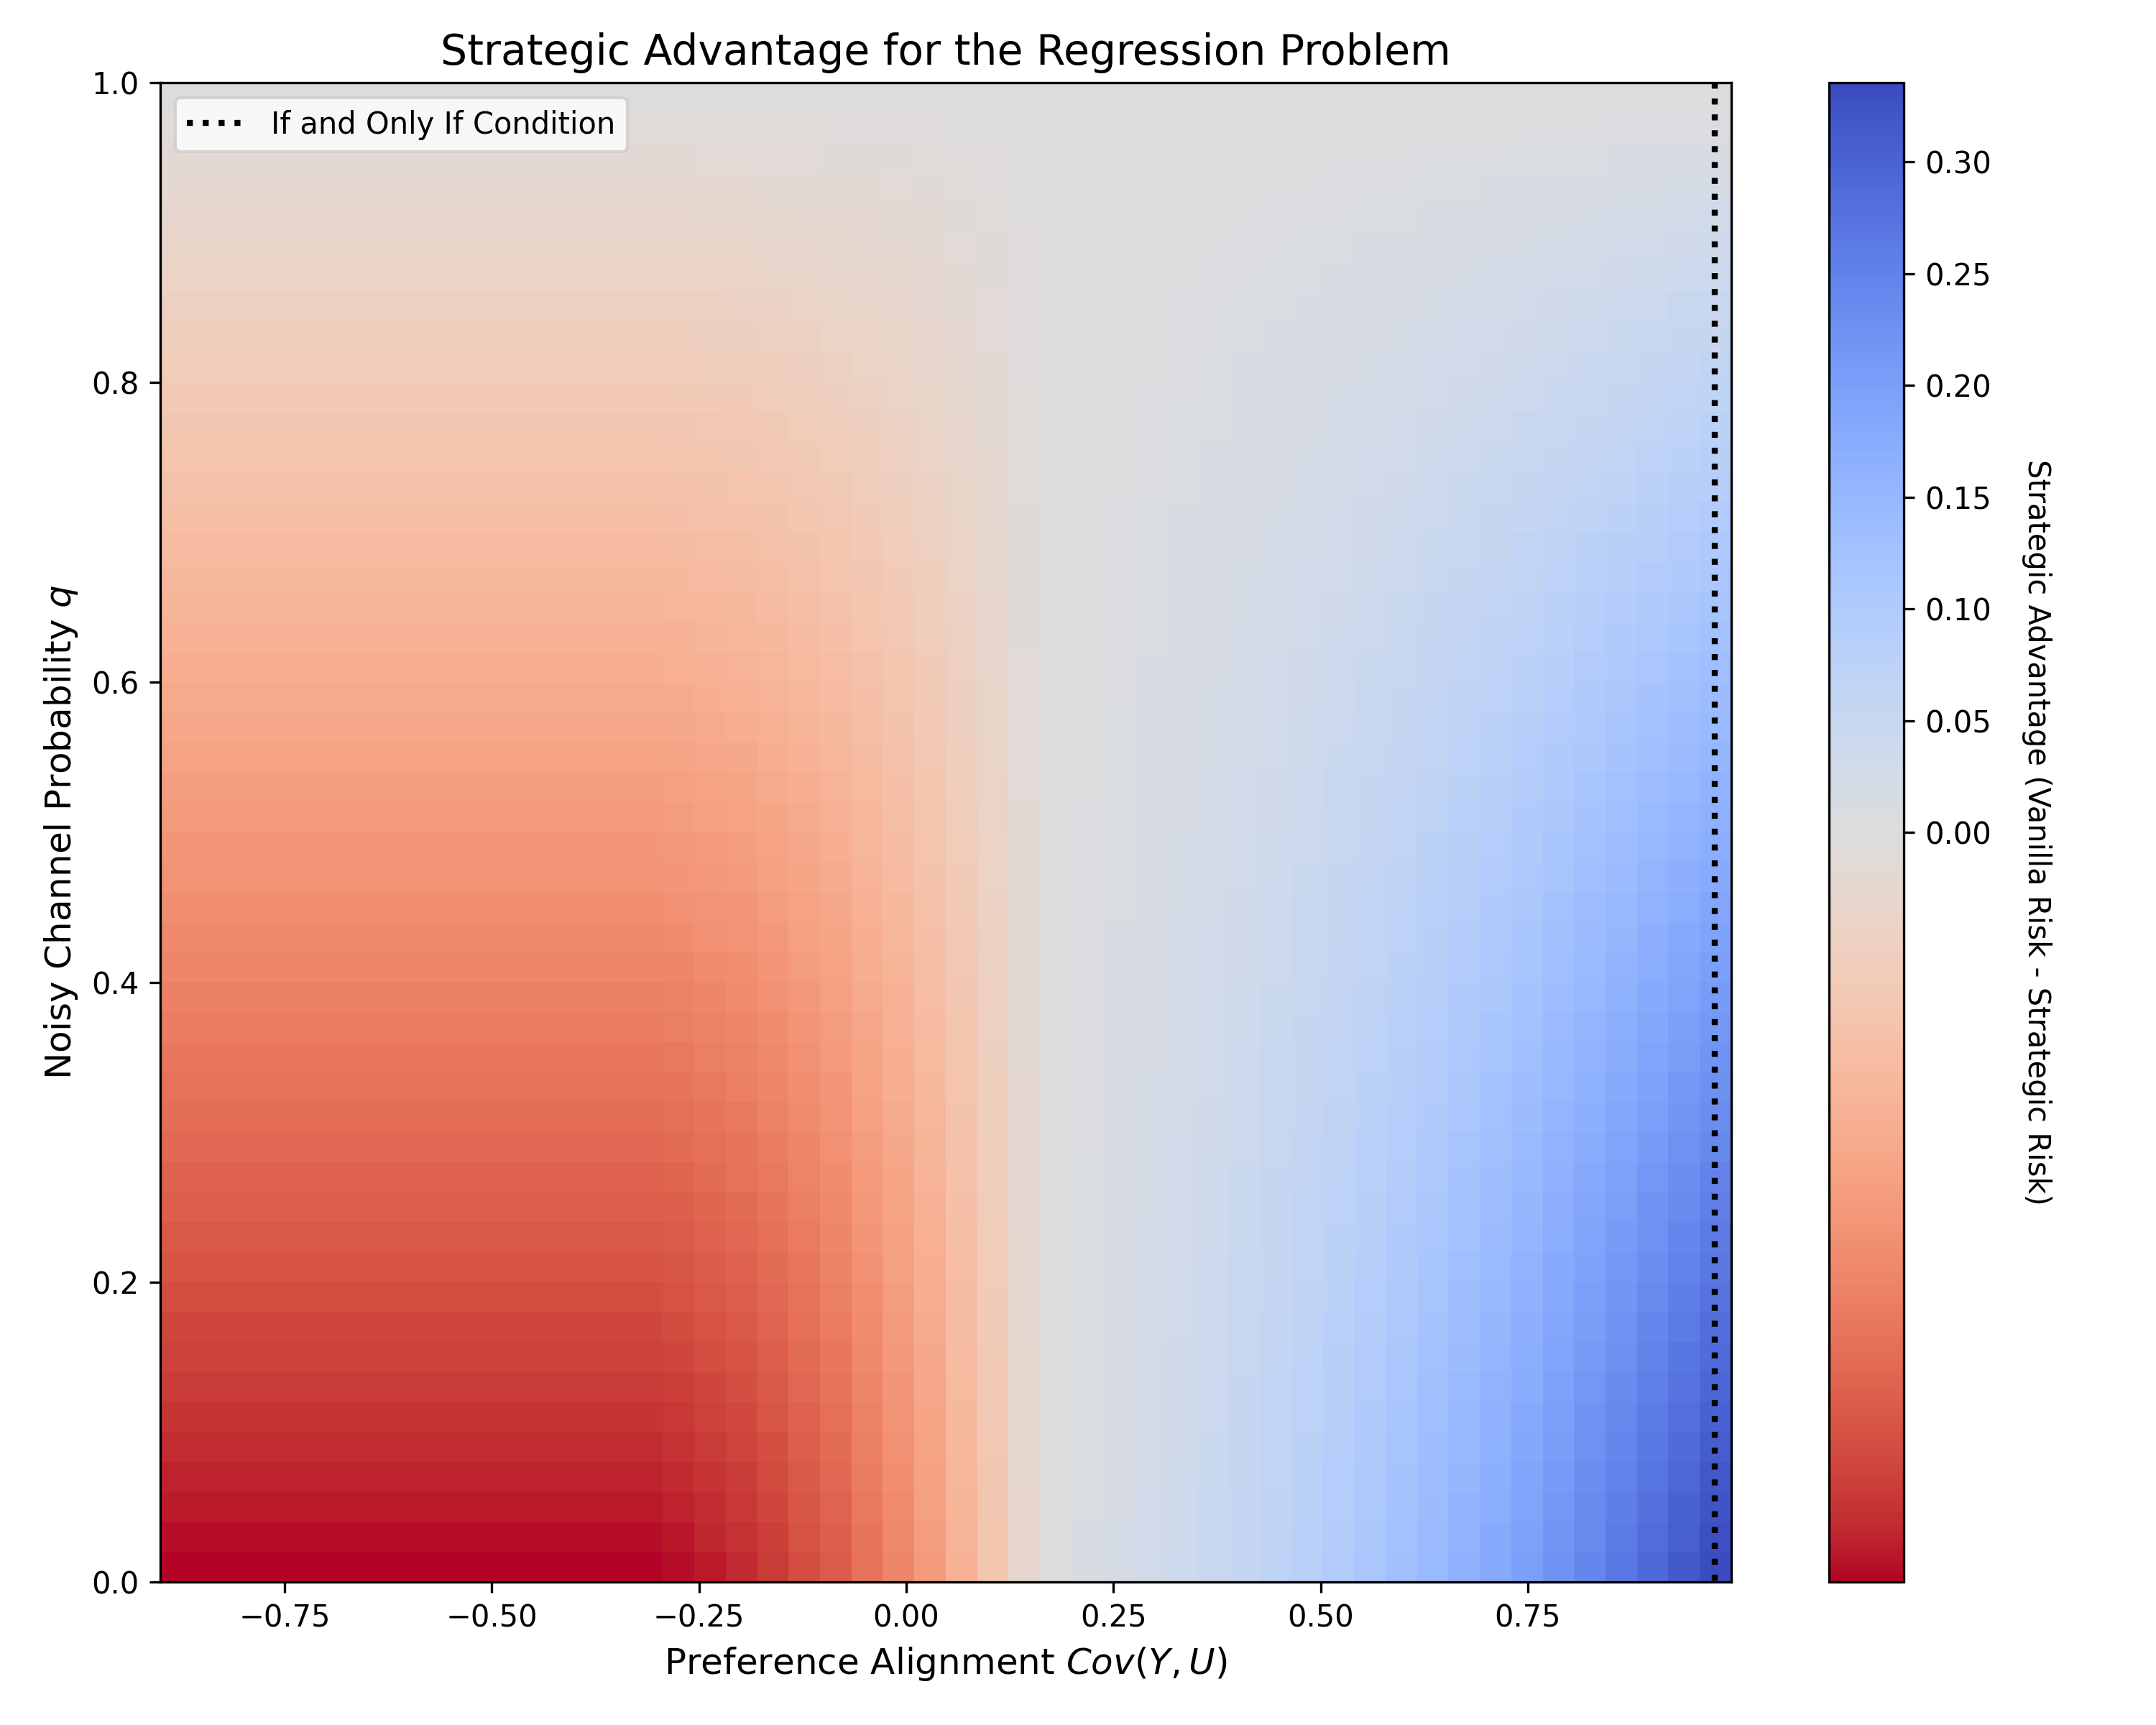
\includegraphics[width=\linewidth]{figures/regression_strategic_advantage.png}
  \caption{Heatmap of the strategic advantage ($R_V^\star(q) - R_S^\star(q)> 0$) for the general regression setup. The parameter space sweeps the noisy channel probability $q$ along the y-axis and the preference alignment $\Cov(Y,U)$ along the x-axis. The dotted black contour delineates the region where the sufficiency condition is met.}
  \label{fig:regression_conditions}
\end{figure}

To numerically verify these theoretical results, we simulate a regression environment using a family of zero-mean Gaussian distributions for $(X, Y, U)$ with unit marginal variances. We fix $\Cov(X,Y) = \Cov(X,U) = 0.2$ across this family, while $\Cov(Y,U)$ serves as the varying parameter. To explore the parameter space, we sweep the channel noise probability $q \in [0, 1]$ and the alignment $\Cov(Y,U) \in [-1, 1]$. At each point on the grid, the Receiver's risk is minimized over a range of weights $b$ to calculate the strategic risk $R_S$. As demonstrated in Fig.~\ref{fig:regression_conditions}, the analytical boundary reliably delineates the regions of strategic advantage.

